\chapter{Classification Trees}
\label{ch:classification-trees}

In the previous lesson, we used a classification tree,
\marginnote{Classification trees were hugely popular in the early years of machine learning, when they were first independently proposed by the engineer Ross Quinlan (C4.5) and a group of statisticians (CART), including the father of random forests Leo Brieman.}
one of the oldest, but still popular, machine learning methods. We like it since the method is easy to explain and gives rise to random forests, one of the most accurate machine learning techniques (more on this later). So, what kind of model is a classification tree?

Let us load \textit{iris} data set, build a tree (widget \widget{Tree}) and visualize it in a \widget{Tree Viewer}.

\begin{figure}[h]
    \centering
    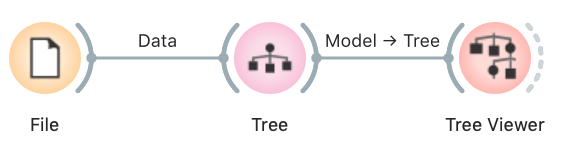
\includegraphics[scale=0.4]{workflow-tree-viewer.png}
\end{figure}

\begin{figure*}[h]
    \vspace{-0.4cm}
    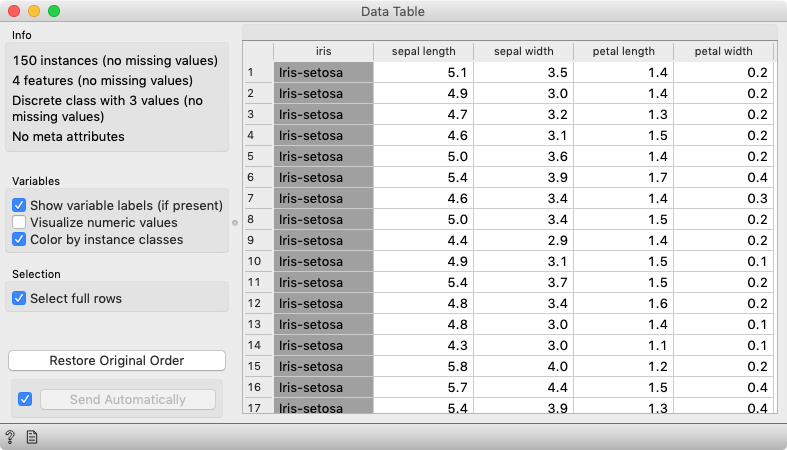
\includegraphics[scale=0.35]{iris-data.png}
    \label{fig:classification-predictions}
\end{figure*}

\begin{wrapfigure}{o}{1.0\textwidth}
    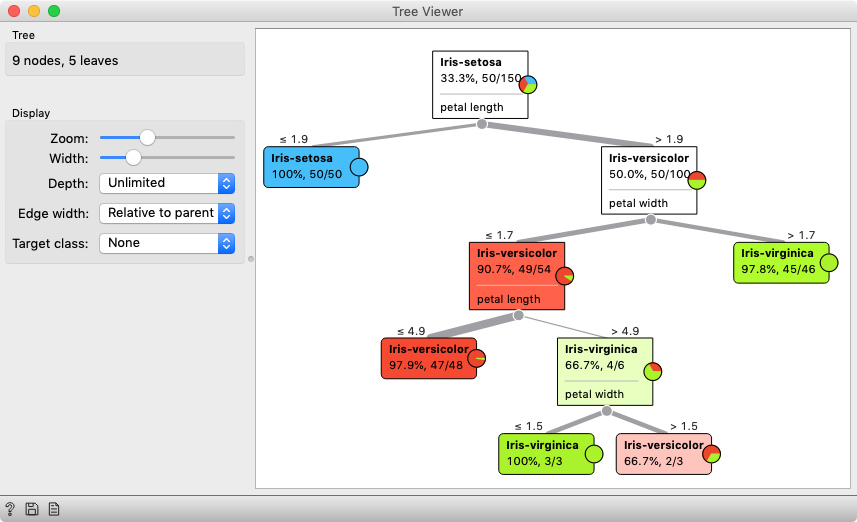
\includegraphics[scale=0.35]{tree-viewer.png}
    \label{fig:classification-predictions}
\end{wrapfigure}

We read the tree from top to bottom. Looks like the column \textit{petal length} best separates the iris variety \textit{setosa} from the others, and in the next step, \textit{petal width} then almost perfectly separates the remaining two varieties.

Trees place the most useful feature at the root. What would be the most useful feature? The feature that splits the data into two purest possible subsets. It then splits both subsets further, again by their most useful features, and keeps doing so until it reaches subsets in which all data belongs to the same class (leaf nodes in strong blue or red) or until it runs out of data instances to split or out of useful features (the two leaf nodes in white).

We still have not been very explicit about what we mean by "the most useful" feature. There are many ways to measure the quality of features, based on how well they distinguish between classes. We will illustrate the general idea with information gain. We can compute this measure in Orange using the \widget{Rank} widget\marginnote{The \widget{Rank} widget can be used on its own to show the best predicting features. Say, to figure out which genes are best predictors of the phenotype in some gene expression data set.}, which estimates the quality of data features and ranks them according to how informative they are about the class. We can either estimate the information gain from the whole data set, or compute it on data corresponding to an internal node of the classification tree in the \widget{Tree Viewer}. In the following example we use the \textit{Sailing} data set.

\begin{figure}[h]
    \centering
    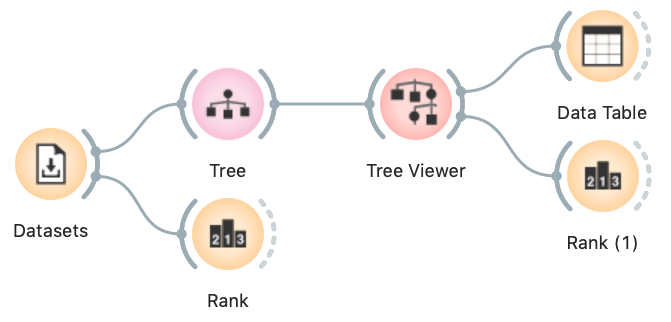
\includegraphics[scale=0.4]{workflow-rank.png}
    \caption{The \widget{Datasets} widget is set to load the \textit{Sailing} data set. To use the second \widget{Rank}, select a node in the \widget{Tree Viewer}.}
\end{figure}

Besides the information gain, \widget{Rank} displays several other measures (including Gain Ratio and Gini), which are often quite in agreement and were invented to better handle discrete features with many different values.

\begin{figure}[h]
    \centering
    \vspace{-0.2cm}
    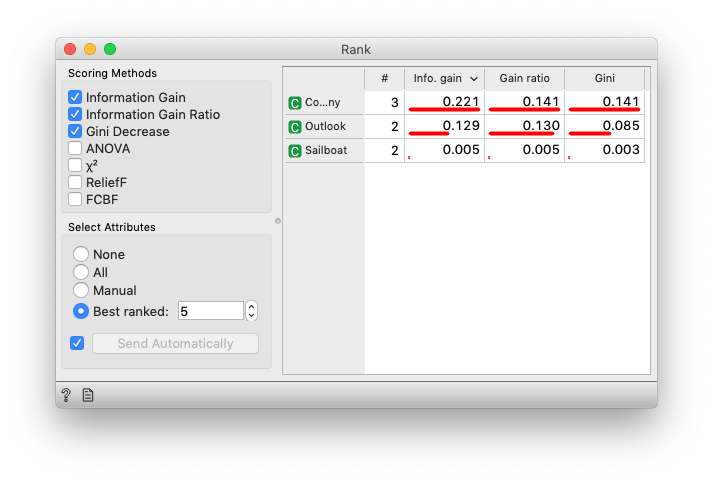
\includegraphics[scale=0.4]{rank.png}
    \caption{For the whole \textit{Sailing} data set, \textit{Company} is the most class-informative feature according to all measures shown.}
\end{figure}

\newpage

Here is an interesting combination of a \widget{Tree Viewer} and a \widget{Scatter Plot}. This time, use the \textit{Iris} data set. In the \widget{Scatter Plot}, we first find the best visualization of this data set, that is, the one that best separates the instances from different classes. Then we connect the \widget{Tree Viewer} to the \widget{Scatter Plot}. Data instances (particular irises) from the selected node in the \widget{Tree Viewer} are shown in the \widget{Scatter Plot}.

\begin{figure}[h]
    \centering
    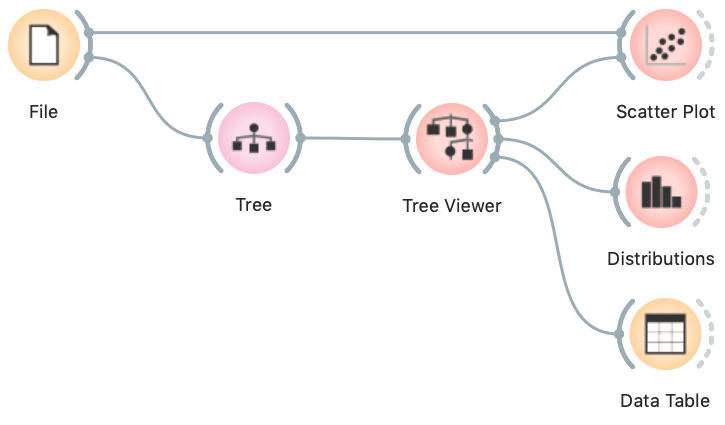
\includegraphics[scale=0.4]{workflow-inspection.png}
    \caption{Careful, the \widget{Data} widget needs to be connected to the \widget{Scatter Plot}'s \textit{Data} input, and \widget{Tree Viewer} to the \widget{Scatter Plot}'s \textit{Data Subset} input.}
\end{figure}

Just for fun, we have included a few other widgets in this workflow. In a way, a \widget{Tree Viewer} behaves like \widget{Select Rows}, except that the rules used to filter the data are inferred from the data itself and optimized to obtain purer data subsets.

\begin{figure*}[h]
  \infinitewidthbox{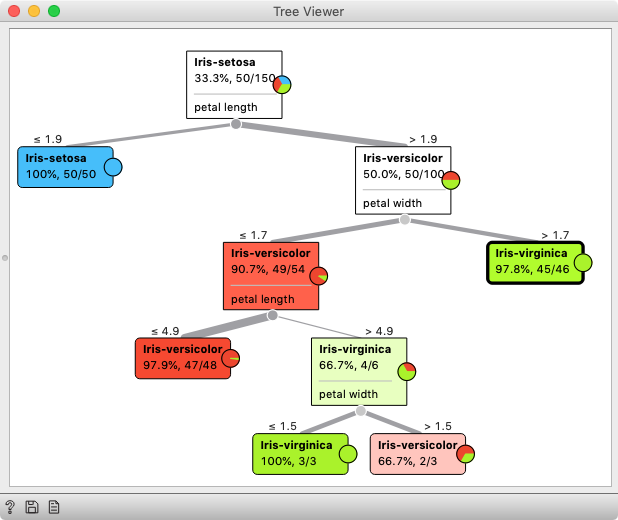
\includegraphics[scale=0.35]{tree-viewer-selection.png} 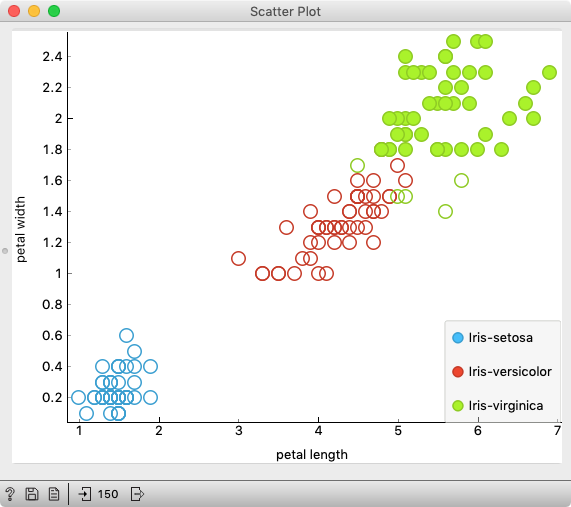
\includegraphics[scale=0.35]{scatter-plot-subset.png}}
  \caption{In the \widget{Tree Viewer} we selected the rightmost node. All data instances coming to the selected node are highlighted in \widget{Scatter Plot}.}
\end{figure*}

Wherever possible, visualizations in Orange are designed to support selection and passing of the data that applies to it. Finding interesting data subsets and analyzing their commonalities is a central part of explorative data analysis, a data analysis approach favored by the data visualization guru Edward Tufte.